\subsubsection{The Sod Problem}\label{ss:Sod}

In 1976, Sod\cite{sod1} published a technical report detailing his implementation of Glimm's method\cite{glimm} for solving the hyperbolic equations for Riemann problems using Godunov iteration \cite{godunov}.  He presented results for three test cases, the initial conditions for each arrangement is shown in Figure~\ref{fig:shockTube}  and in Table~\ref{tab:sodIC}.  In all cases, the ideal gas ratio of specific heats, $\gamma = 5/3 = \gamma_l = \gamma_r$.

\begin{table}[h!]
 \begin{center}
  \caption{Initial conditions for Sod's three test cases.}
  \label{tab:sodIC}
  \begin{tabular}{|c|ccc|cccc|cccc|} \hline
   \textbf{Case} & \multicolumn{3}{c|}{\textbf{Domain}} & \multicolumn{4}{c|}{\textbf{Left Gas}} & \multicolumn{4}{c|}{\textbf{Right Gas}} \\ \hline
   \multirow{2}{*}{$Sod_1$} & $x_L$ & $x_D$ & $x_R$ & $\rho$ & $u$ & $P$ & $\gamma$ & $\rho$ & $u$ & $P$ & $\gamma$ \\ \cline{2-12}
   \multicolumn{1}{|c|}{} & 0. & 0.75 & 1.  & 1. & 0. & 1. & 5/3 & 1. & 0. & 0.1 & 5/3 \\ \hline
   $Sod_2$  & 0. & 0.5 & 1.  & 1. & 0. & 1. & 5/3 & 0.125 & 0. & 0.1 & 5/3 \\ \hline
   $Sod_3$ & 0. & 0.3 & 1.  & 1. & 0. & 666.7 & 5/3 & 0.001 & 0. & 0.00000667 & 5/3 \\ \hline
   $Sod_{3-Mod}$ & 0. & 0.3 & 1.  & 1. & 0. & 66.67 & 5/3 & 0.2 & 0. & 0.06667 & 5/3 \\ \hline
  \end{tabular}
 \end{center}
\end{table}

\paragraph{Case $Sod_1$}

In this case, Sod examined the effects of shock and rarefaction waves reflecting off the walls at $x_L = 0$ and $x_R = 1$ using symmetry boundary conditions.  At  $t = 0$, the gases are separated by a diaphragm at $x_D = 0.75$. His results are at three simmulation times: $t = 0.1780$, $0.8526$, and $1.0210$. In the first case shown in Figure~\ref{fig:Sod1-1}, Flexi was run using a mesh generated with HOPR using the input deck listed in \ref{ssec:hoprin-sod1} and Flexi executed using the input listed in \ref{ssec:flexiin-sod1}. Table~\ref{tab:sod1Eps} shows the average error for the Flexi solution is less than $0.002$.

\begin{figure}[h!]
 \centering
 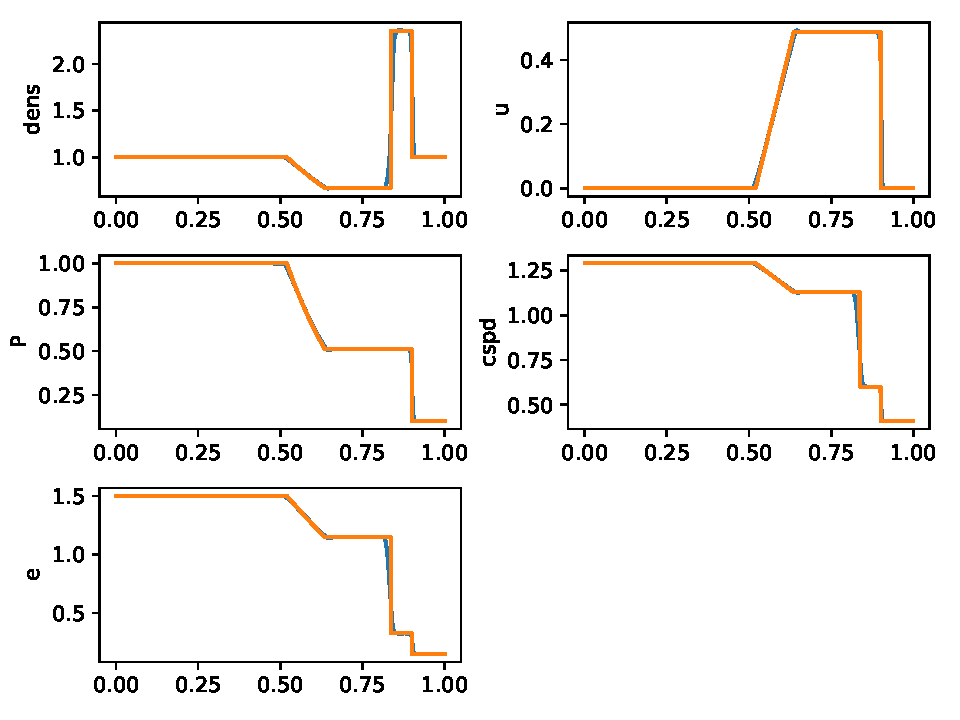
\includegraphics[scale=0.8]{figures/sod1-BC9-PV.pdf}
 \caption{$sod_1$ results for $t = 0.1780$ compared to the exact solution. Flexi data are the blue curves and exact are red.}
 \label{fig:Sod1-1}
\end{figure}

\begin{table}[h!]
 \centering
 \begin{tabular}{|c|c|} \hline
   Variable & $\bar{\epsilon}$ \\ \hline \hline
   $\rho$ & 0.00156 \\
   $v_x$  & 0.00071 \\
   $u$     & 0.00112 \\
   $P$     & 0.00059 \\ \hline
 \end{tabular}
 \caption{Average error for the $Sod_1$ Problem}\label{tab:sod1Eps}
\end{table}


\paragraph{Case $Sod_2$}

In a second case, Sod examined the effects of shock and rarefaction waves reflecting off the walls at $x_L = 0$ and $x_R = 1$ with $x_D = 0.5$ using inflow/outflow boundary conditions.  His results are at $t = 0.2746$. In this case shown in Figure~\ref{fig:Sod2-BC2}, Flexi was run using a mesh generated with HOPR using the input deck listed in \ref{ssec:hoprin-sod2-BC2} and Flexi executed using the input listed in \ref{ssec:flexiin-sod2-BC2}. The flexi results are nearly identical to the exact solution, however it is noted the these results are dramatically different from the results shown in Figure 11 of \cite{sod1}.

\begin{figure}[h!]
 \centering
 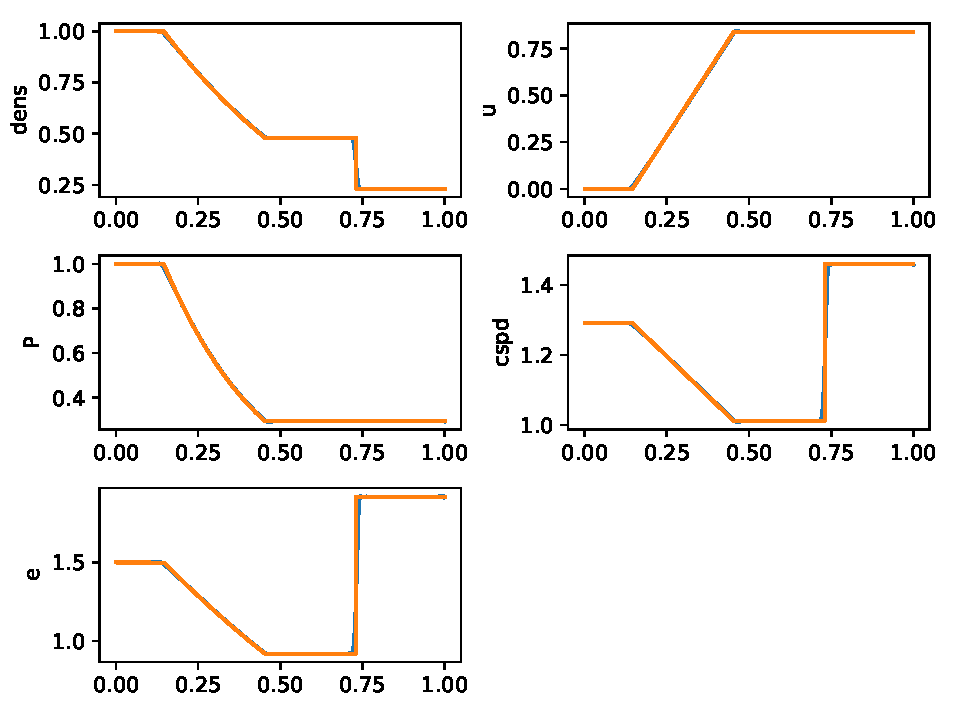
\includegraphics[scale=0.8]{figures/sod2-BC2-PV.pdf}
 \caption{$sod_2$ results for $t = 0.2746$ with inflow/outflow boundary conditions as compared to the exact solution (red curves). Flexi data are in blue.}
 \label{fig:Sod2-BC2}
\end{figure}

If instead of inflow/outflow boundary condition they are changed to symmetry conditions, the flexi results compared with the exact solution are shown in Figure~\ref{fig:Sod2-BC9}.  These results show the effect of the shock reflecting from the $x_R$ boundary. Note that the exact solution has only inflow/outflow boundaries. Flexi was run using a mesh generated with HOPR using the input deck listed in \ref{ssec:hoprin-sod2-BC9} and Flexi executed using the input listed in \ref{ssec:flexiin-sod2-BC9}.

\begin{figure}[h!]
 \centering
 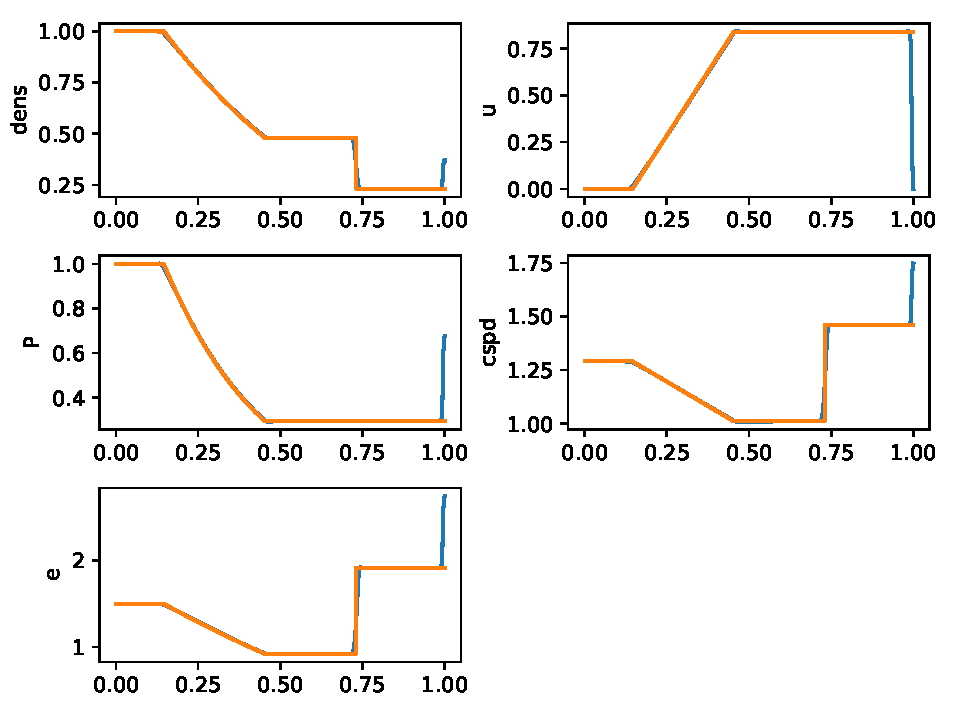
\includegraphics[scale=0.8]{figures/sod2-BC9-PV.pdf}
 \caption{$sod_2$ results for $t = 0.2746$ with symmetry boundary conditions as compared to the exact solution (red curves). Flexi data are blue curves. Note the effect of the symmetry condition at the right boundary in the flexi results and that the exact solution does not have symmetry boundary conditions.}
 \label{fig:Sod2-BC9}
\end{figure}

Table~\ref{tab:sod2Eps} shows the average error for the Flexi solution is less than $0.0015$.

\begin{table}[h!]
 \centering
 \begin{tabular}{|c|c|} \hline
   Variable & $\bar{\epsilon}$ \\ \hline \hline
   $\rho$ & 0.00065 \\
   $v_x$  & 0.00135 \\
   $u$     & 0.00147 \\
   $P$     & 0.00091 \\ \hline
 \end{tabular}
 \caption{Average error for the $Sod_2$ Problem}\label{tab:sod2Eps}
\end{table}

\paragraph{Case $Sod_3$: Symmetry Boundary Conditions}

In a third case (\textit{c.f.:} \ref{tab:sodIC}), Sod examined a challenging Rieman problem in the usual domain $x_L = 0$ and $x_R = 1$ with $x_D = 0.3$ using symmetry boundary conditions.  Here, the Left gas has density $\rho_L = 1.,$ and Right density $\rho_R = 0.001$ and Left pressure $P = 6.6667e^{2}$ and Right pressure $P_R = 6.6667e{-6}$.  This is essentially propagation of an ideal gas into a vacuum.

Flexi was unable to complete these calculations due to NaN's being generated in the time discretization step.  However, attempts were made to run flexi for less extreme initial conditions: $\rho_L = 1.$, $\rho_R = 0.2$ and $P_L = 66.667$, $P_R = 0.066667$. Results are at $t = 0.01812$.  as shown in Figure~\ref{fig:multiSod3-BC9}. Flexi was run using a mesh generated with HOPR using the input deck listed in \ref{ssec:hoprin-sod3-BC9} and Flexi executed using the input listed in \ref{ssec:flexiin-sod3-BC9}.

\begin{figure}[h!]
 \centering
 %\includegraphics[scale=0.8]{figures/sod3-BC9-g-5o3-t-1812o10000-x0-3o10.pdf}
 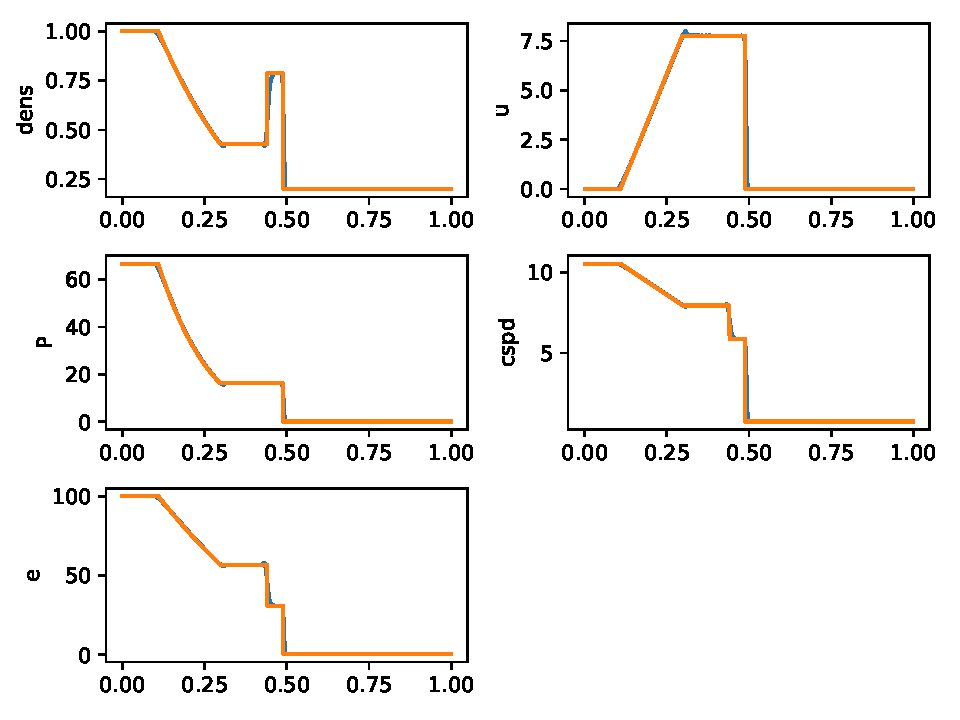
\includegraphics[scale=0.8]{figures/sod3-BC9-PV.pdf}
 \caption{$sod_{3-mod}$ results for the modified input discussed above at $t = 0.01812$ (blue curves) compared to the exact solution (red curves).}
 \label{fig:multiSod3-BC9}
\end{figure}

Table~\ref{tab:sod3Eps} shows the average error for the Flexi solution is less than $0.007$.

\begin{table}[h!]
 \centering
 \begin{tabular}{|c|c|} \hline
   Variable & $\bar{\epsilon}$ \\ \hline \hline
   $\rho$ & 0.00092 \\
   $v_x$  & 0.00330 \\
   $u$     & 0.00712 \\
   $P$     & 0.00425 \\ \hline
 \end{tabular}
 \caption{Average error for the $Sod_{3-mod}$ Problem}\label{tab:sod3Eps}
\end{table}

\paragraph{Conclusions}\label{pp:sodConc}
For the cases presented in this section, Flexi was able to very nearly reproduce the exact solutions. These results ran with the number of Finite Volume zones at 2 to 4\% of the total zones; those zones handling the shock/rarefaction dynamics.
